% group articles by domain 
% for every article write a short summary of its relevant features
% and add an illustrative picture
% then criticize the presented solutions

\subsection{Multimodal Interfaces}

In order to obtain an immersive experience, there's a number of hardware
setups commonly available:

\begin{description}
	\item[Head Mounted Display (HMD)] --
	  Head mounting displays are glass shaped devices, projecting a pair of stereo
	  transformed images to the user's retinas.
	  They normally feature a gyroscope or similar apparatus to measure head orientation and tilt.
	  There are two kinds of HMDs: in the former the images are projected in small opaque screens;
	  in the latter the projected surface is translucid, allowing blending of real and virtual worlds.
	  
		Using a head mounted display has the benefit of sticking to the user's head
		and detecting head orientation.
		On the other hand each HMD serves one single user.
		Additionally, most users report suffering from fatigue after long periods of
		usage \cite{VREDUC} and it has limited resolution.
		Opaque HMDs have and additional downside of users being unable to see the real world, 
		which can be confusing as noted by \cite{VANDERPOL}
			
	\item[Cave Automatic Virtual Environment (CAVE)] --
	  A CAVE is an immersive virtual reality environment where projectors are directed to four,
	  five or all the six walls of a room-sized cube.
	  
		It shares the benefit of enclosing the user's viewing area with HMDs.
		Has a better resolution though.
		The downside is the small number of simultaneous users who can experience the CAVE at the same time.
	
	\item[Power Wall] --
	  A power wall is a large surface, usually planar, filled by an image.
	  The whole image projection is responsibility of a cluster of projectors set up in a wall.
	  Each projector renders part of the surface and the border between projections is ideally minimal.
	  Each projector is controlled by an independent computer.
	  
		Its size and resolution depend entirely on the setup, but normally a wall offers high resolution
		(depends on the number of projectors in the grid and each projector's resolution).
		Due to the large surface of the wall, several users may be served as once. Another benefit
		is users freedom of movement due to users not carrying wires. \cite{INTTABLE}
		The downside is users having to face the wall to experience the image entirely.
\end{description}

\begin{figure}[!ht]
	\centering
	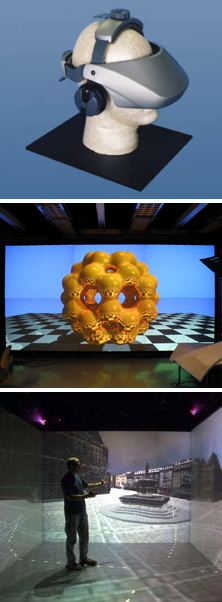
\includegraphics[width=11cm]{gfx/hmd-cluster-cave.png}
	\caption{HMD, Wall, CAVE}
	\label{FIG-HMD-CLUSTER-CAVE}
\end{figure}

Any of these setups is suitable for single user interaction.
In case of a reviewing session, in which at least two participants are required,
CAVE or Wall are better suited, since they alone offer a solution for a small group.

Using a Wall or CAVE presents other challenges: the computers responsible for
generating each projectors' images must be synchronized, its' color parameters calibrated,
the viewport must be well cropped, etc.
Several systems exist capable of delivering high performance 3D graphics and
offering the features mentioned above.
Based on scene graphs there are two well known solutions:
OpenSceneGraph\cite{SITE-OSG}
and
OpenSG\cite{SITE-OPENSG}.

\subsubsection{Studies}


\subsubsection{Systems}

Kaufmann and Schmalstieg \cite{VREDUC} propose a collaborative Augmented Reality (AR)
system  named Construct3D for teaching high school students 3D modeling.
It supports two users wearing a see-through head-mounted display and with tracked head and pens.

Precise geometry construction is pointed out as difficult to accomplish in 3D space by direct
manipulation in 6 degrees of freedom due to tracking inaccuracies, lack of hand-eye coordination,
hand tremor and difficulties in precisely locating a 3D point presented with a fixed-focus stereoscopic.
This problem was solved by restricting the user's input to two dimensions and
providing grids and snapping functions to enable precision modeling.

Kaufmann and Schmalstieg give low importance to environment coordinates as indications of
position in space in a dynamic construction scenario.

\begin{figure}[!ht]
	\centering
	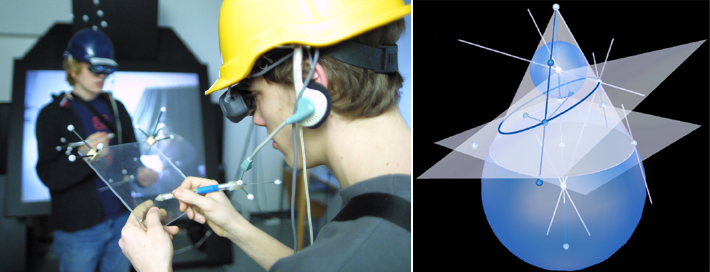
\includegraphics[width=10cm]{gfx/vreduc.png}
	\caption{Construct3D: user interface (left); proof that the intersection of plane
and cone are either ellipse, hyperbola or parabola -- planes can be dynamically moved (right)}
	\label{FIG-VREDUC}
\end{figure}

Wesche and Seidel \cite{FREED} present a sketching system named FreeDrawer.
It allows curve drawing and editing. The user wears a head-mounted display, handles a stylus
with the dominant hand with which the drawing is made. The remaining hand controls positioning
and orientation. The system's purpose is to allow conceptual design creation.
The system hides its internal complexity (B-spline curves and Catmull-Clark surfaces).
It estimates connectivity between curves by a threshold maximum distance.

%\cite{INTTABLE}
%powerwall interaction problems, interaction table as solution

%\cite{TANINT}
%digital tape drawing and eraser pen to design 3d curves for automotive design

\cite{GROSS}
3D modeling on large displays: construction planes, tape drawing, 2 hand interaction

Cao and Balakrishnan propose themselves in devising an input technique to serve
large display interaction. VisionWand is a plastic rod with colored ends, tracked by
two low budget cameras. The tracking results in a 3D ray. Since the rod has no
electronics to support button clicking or similar actions, a set of gestures was
defined to allow user command input (see Fig. \ref{FIG-VISIONWAND}).
VisionWand points out interesting functionality for the tracking data:
pointing with different ends of the wand invokes either manipulation or query actions,
while parallel posture activates a menu.
Distance from wand to screen serves as zooming factor where applicable.
In pie menus, wand orientation controls option selection.


\begin{figure}[!ht]
	\centering
	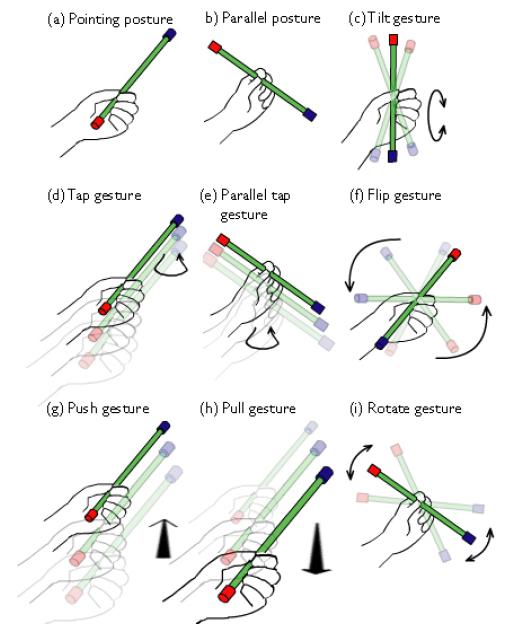
\includegraphics[width=4.5cm]{gfx/visionwand.png}
	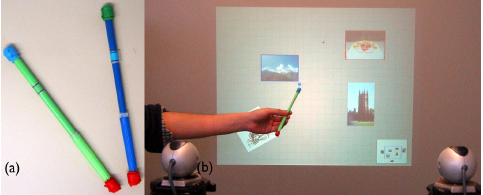
\includegraphics[width=7.5cm]{gfx/visionwand2.png}
	\caption{VisionWand: set of gestures(left); wands and hardware setup (right)}
	\label{FIG-VISIONWAND}
\end{figure}


\cite{WAND}
tracked wand interaction - postures, gestures

\cite{GESREC}
hand tracking for gesture recognition. Forward HMMs and NNs tested.



\subsection{Sketching}
\subsubsection{Beautification}
\subsubsection{2D to 3D Reconstruction}
\subsubsection{Suggestive Interfaces and Grammars}

\subsection{Navigation}

\subsection{Knowledge Representation}

\subsection{Text Entry}

